\documentclass{template/v1}

% Define Metadata
\Title{Thiết kế và triển khai hệ thống dự đoán lưu lượng và điều khiển định tuyến chủ động cho mạng nhà cung cấp dịch vụ Internet dựa trên mạng điều khiển bằng phần mềm, sử dụng học liên kết và học tăng cường.}
\Title[en]{Design and Implementation of a Traffic Prediction and Proactive Routing Control System for SDN-Based ISP Networks Using Federated Learning and Reinforcement Learning}

\Author{Đào Anh Kiệt}{23520810}
\Author{Trần Bùi Nhật Nguyên}{23521059}

\Advisor{ThS. Nguyễn Khánh Thuật}
% \Advisor{PGS.TS. Hoàng Văn B}

\Faculty{Khoa Mạng máy tính và Truyền thông}
\ThesisFromDate{01/08/2026}   %Thời gian bắt đầu thực hiện KLTN dd/mm/yyyy
\ThesisToDate{27/12/2026}     % %Thời gian kết thúc thực hiện KLTN dd/mm/yyyy


\begin{document}
\printinfo

\vspace*{3ex}

\section{Tổng quan đề tài:}
\label{sec:tong-quan-de-tai}
% Sinh viên cần nêu rõ các đề tài, sản phẩm liên quan đã được nghiên cứu hoặc đã có trên thị trường trước thời điểm hiện tại và nêu thực trạng của chúng, để từ đó nêu bật được lý do thực hiện nghiên cứu trong KLTN này

Sự phát triển mạnh mẽ của các dịch vụ số như điện toán đám mây, IoT, 5G, trí tuệ nhân tạo và truyền phát video trực tuyến đã làm lưu lượng mạng Internet tăng nhanh, buộc các nhà cung cấp dịch vụ Internet (ISP) phải không ngừng mở rộng hạ tầng và ứng dụng các công nghệ hiện đại như Software-Defined Networking (SDN) để nâng cao hiệu quả quản lý mạng. Tuy nhiên, sự gia tăng lưu lượng cùng tính biến động cao của các ứng dụng hiện đại đã làm phát sinh nhiều vấn đề như tắc nghẽn mạng, mất cân bằng tải, gia tăng độ trễ và suy giảm chất lượng dịch vụ. Trong khi đó, các cơ chế định tuyến và điều khiển lưu lượng chủ yếu dựa trên trạng thái mạng hiện tại thường chỉ phản ứng sau khi lưu lượng thay đổi hoặc tình trạng quá tải bắt đầu xảy ra. Điều này làm hạn chế khả năng chủ động điều chỉnh lưu lượng và phòng tránh tắc nghẽn trước khi xảy ra. Vì vậy, việc nghiên cứu các giải pháp điều khiển lưu lượng có khả năng dự đoán xu hướng lưu lượng trong tương lai và sử dụng thông tin dự đoán để hỗ trợ quyết định Traffic Engineering theo hướng chủ động là cần thiết nhằm nâng cao hiệu quả sử dụng tài nguyên, giảm tắc nghẽn và cải thiện chất lượng dịch vụ trong mạng ISP.

Để giải quyết các vấn đề trên, nhiều giải pháp tối ưu hóa điều khiển lưu lượng đã được nghiên cứu và triển khai như Traffic Engineering, Software-Defined Networking (SDN) và các thuật toán học máy (Machine Learning). Gần đây, các hướng nghiên cứu tập trung vào việc ứng dụng trí tuệ nhân tạo nhằm dự đoán lưu lượng mạng và tối ưu quyết định định tuyến, trong đó Federated Learning (FL) được sử dụng để huấn luyện mô hình dự đoán trên dữ liệu phân tán mà không cần chia sẻ dữ liệu gốc, còn Reinforcement Learning (RL) được áp dụng để học và lựa chọn đường truyền tối ưu theo trạng thái mạng. Tuy nhiên, phần lớn các nghiên cứu hiện nay chỉ tập trung vào từng kỹ thuật riêng lẻ hoặc chưa khai thác hiệu quả sự kết hợp giữa FL và RL trong môi trường mạng ISP dựa trên SDN. Đồng thời, khả năng điều khiển lưu lượng theo hướng chủ động dựa trên dự đoán lưu lượng tương lai vẫn còn là một khoảng trống nghiên cứu cần được tiếp tục khai thác.


\begin{figure}[!h]
    \centering
    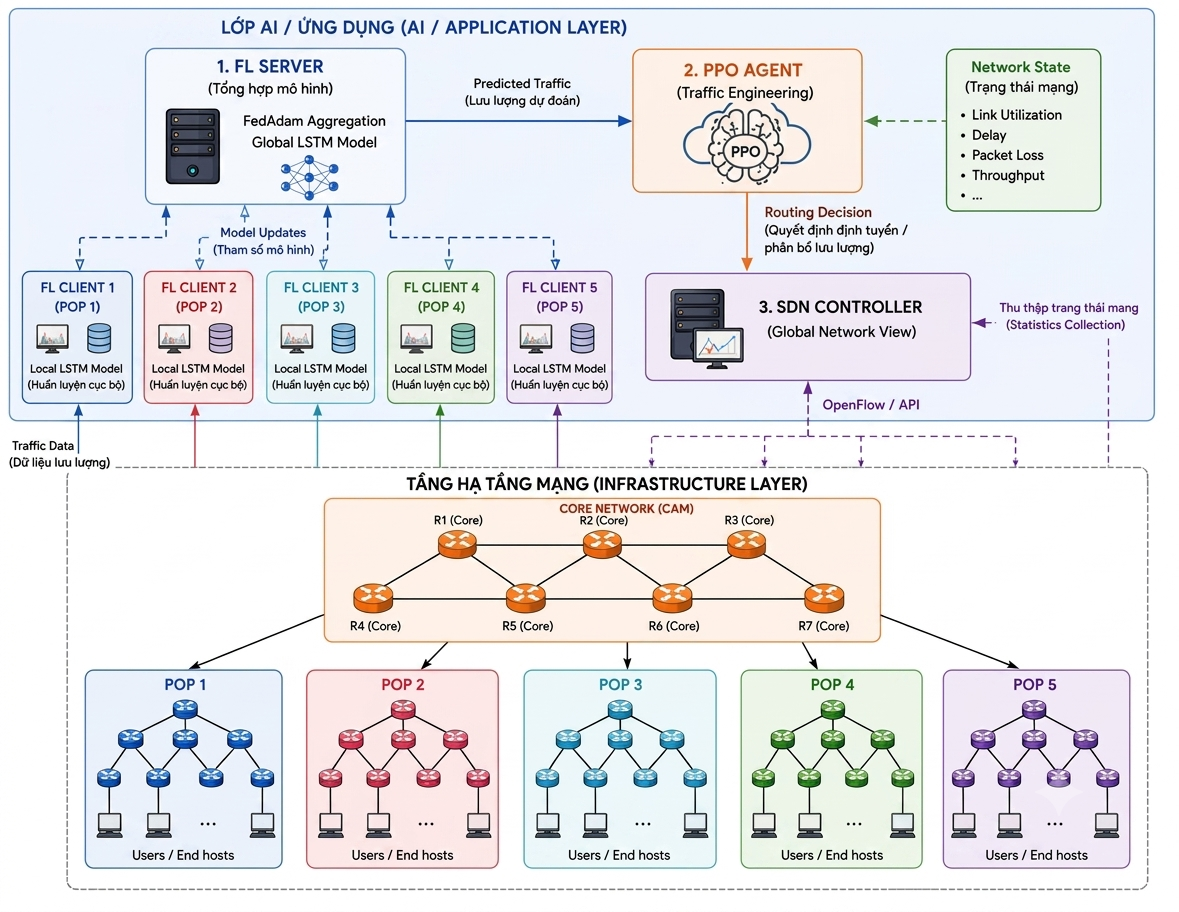
\includegraphics[width=0.75\linewidth]{Figures/Hệ thống đề xuất.png}
    \caption{Hệ thống đề xuất}
    \label{fig:proposed-system}
\end{figure}

Xuất phát từ những hạn chế trên, đề tài đề xuất một giải pháp điều khiển lưu lượng chủ động trong mạng ISP dựa trên SDN bằng cách kết hợp Federated Learning và Reinforcement Learning. Trong kiến trúc đề xuất, FL được sử dụng tại các miền hoặc nút mạng có dữ liệu lưu lượng phân tán để huấn luyện mô hình dự đoán lưu lượng mà không cần tập trung dữ liệu gốc. Các FL Client thực hiện huấn luyện cục bộ và gửi tham số mô hình đến FL Server để tổng hợp thành mô hình toàn cục. Mô hình toàn cục sau đó được sử dụng để dự đoán xu hướng lưu lượng trong tương lai. Kết quả dự đoán được kết hợp với trạng thái mạng hiện tại và cung cấp cho tác tử RL để thực hiện Traffic Engineering, lựa chọn tuyến truyền hoặc phương án phân bổ lưu lượng phù hợp. Quyết định của tác tử RL được chuyển đến bộ điều khiển SDN để thực thi trên các thiết bị mạng, qua đó hướng đến giảm tắc nghẽn, cân bằng tải, cải thiện độ trễ và nâng cao hiệu quả sử dụng tài nguyên mạng.

FL được nghiên cứu nhằm hỗ trợ dự đoán lưu lượng trong các mạng phân tán mà không cần chia sẻ dữ liệu gốc giữa các miền mạng. Li và cộng sự \cite{li2024core} đã kết hợp Vertical Federated Learning và Split Learning để dự đoán lưu lượng mạng lõi, trong khi Gao và cộng sự \cite{gao2024communication} đề xuất cơ chế giảm chi phí truyền thông trong quá trình huấn luyện FL. Zhao và cộng sự \cite{zhao2024federated} áp dụng FL kết hợp Graph Neural Network cho dự đoán lưu lượng trong mạng tích hợp vệ tinh – mặt đất. Tuy nhiên, các nghiên cứu này chủ yếu tập trung vào dự đoán lưu lượng và chưa khai thác kết quả dự đoán để tối ưu quyết định định tuyến.

RL được ứng dụng rộng rãi trong tối ưu định tuyến và điều khiển lưu lượng nhờ khả năng học chính sách tối ưu từ trạng thái mạng. Dake và cộng sự \cite{dake2021traffic} đã tổng quan các phương pháp RL trong Traffic Engineering cho SDN. Al Jameel và cộng sự \cite{aljameel2022reinforcement} sử dụng RL để cải thiện định tuyến cho lưu lượng thời gian thực, trong khi Wang và cộng sự \cite{wang2026deep} kết hợp Deep RL với Graph Multi-Head Attention nhằm nâng cao hiệu quả lựa chọn đường đi. Mặc dù đạt kết quả tốt, các nghiên cứu này chủ yếu dựa trên trạng thái mạng hiện tại và chưa kết hợp thông tin dự đoán lưu lượng để thực hiện điều khiển lưu lượng chủ động.

\begin{table*}[ht]
\centering
\caption{So sánh các công trình nghiên cứu liên quan}
\label{tab:related_work}
\resizebox{\textwidth}{!}{
\begin{tabular}{p{3.2cm}p{3.2cm}p{3.5cm}p{3cm}p{4.8cm}}
\hline
\hline
\textbf{Công trình} &
\textbf{Lĩnh vực} &
\textbf{Hướng tiếp cận} &
\textbf{Mô hình} &
\textbf{Hạn chế} \\
\hline

\citeauthor{li2024core} \cite{li2024core}
&
Traffic Prediction
&
Dự đoán lưu lượng mạng lõi bằng FL
&
Vertical FL + Split Learning
&
Chỉ tập trung dự đoán, chưa tối ưu định tuyến.
\\
\hline

\citeauthor{gao2024communication} \cite{gao2024communication}
&
Traffic Prediction
&
Giảm chi phí truyền thông trong FL
&
Federated Learning
&
Chưa xem xét điều khiển lưu lượng.
\\
\hline

\citeauthor{zhao2024federated} \cite{zhao2024federated}
&
Traffic Prediction
&
Dự đoán lưu lượng mạng di động bằng FL
&
FL + GNN
&
Chưa tích hợp cơ chế định tuyến.
\\
\hline

\citeauthor{aouedi2025deep} \cite{aouedi2025deep}
&
Traffic Prediction
&
Tổng quan các phương pháp DL dự đoán lưu lượng
&
LSTM, GRU, Transformer,...
&
Chỉ tổng hợp nghiên cứu, không đề xuất mô hình mới.
\\
\hline

\citeauthor{dake2021traffic} \cite{dake2021traffic}
&
Traffic Engineering
&
Khảo sát RL trong SDN
&
Q-learning, DQN, PPO,...
&
Không kết hợp dự đoán lưu lượng.
\\
\hline

\citeauthor{aljameel2022reinforcement} \cite{aljameel2022reinforcement}
&
Routing
&
Định tuyến QoS bằng RL
&
Deep Reinforcement Learning
&
Ra quyết định dựa trên trạng thái hiện tại.
\\
\hline

\citeauthor{wang2026deep} \cite{wang2026deep}
&
Routing
&
Tối ưu định tuyến SDN
&
DRL + Graph Attention
&
Chưa sử dụng dự báo lưu lượng.
\\
\hline

\citeauthor{jha2026asynchronous} \cite{jha2026asynchronous}
&
Traffic Engineering
&
Kết hợp FL và RL cho cân bằng tải
&
Federated Reinforcement Learning
&
Tập trung load balancing, chưa nghiên cứu dự đoán lưu lượng.
\\
\hline
\hline
\end{tabular}
}
\end{table*}

\section{Mục tiêu của đề tài:}
\label{sec:muc-tieu-de-tai}
% Nêu cụ thể mục tiêu của KLTN, đặc biệt phải nêu được mục tiêu cải tiến sẽ là gì so với thực trạng nêu trong phần tổng quan đề tài

\subsection*{a) Mục tiêu tổng quát:}
Mục tiêu của đề tài là xây dựng hệ thống dự đoán lưu lượng và điều khiển lưu lượng chủ động trong mạng ISP dựa trên SDN nhằm nâng cao hiệu quả sử dụng tài nguyên mạng, giảm tình trạng tắc nghẽn và cải thiện chất lượng dịch vụ. Hệ thống sử dụng Federated Learning để huấn luyện mô hình dự đoán lưu lượng từ dữ liệu phân tán tại các miền mạng. Kết quả dự đoán lưu lượng trong tương lai được kết hợp với trạng thái mạng hiện tại và cung cấp cho Reinforcement Learning để thực hiện Traffic Engineering, lựa chọn tuyến hoặc phương án phân bổ lưu lượng phù hợp. Các quyết định này được thực thi thông qua bộ điều khiển SDN nhằm điều khiển lưu lượng theo hướng chủ động. Qua đó, hệ thống hướng đến khả năng thích ứng với sự thay đổi của lưu lượng mạng trong khi vẫn đảm bảo không tiết bộ sơ đồ mạng trong các miền mạng.

\subsection*{b) Mục tiêu cụ thể:}
\begin{itemize}
    \item \textbf{Thu thập và tiền xử lý dữ liệu:} lưu lượng mạng từ các bộ dữ liệu công khai hoặc môi trường mô phỏng SDN, đồng thời phân chia dữ liệu theo nhiều miền để mô phỏng kịch bản Federated Learning.

    \item \textbf{Thiết kế và xây dựng hệ thống:} xây dựng kiến trúc điều khiển lưu lượng chủ động trên nền tảng SDN, trong đó các nút hoặc miền mạng thực hiện huấn luyện cục bộ thông qua FL Client, FL Server tổng hợp mô hình dự đoán, mô-đun RL sử dụng kết quả dự đoán kết hợp với trạng thái mạng để thực hiện Traffic Engineering, và SDN Controller thực thi các quyết định điều khiển trên mạng.

    \item \textbf{Xây dựng mô hình dự đoán lưu lượng:} sử dụng Federated Learning để huấn luyện mô hình LSTM trên dữ liệu lưu lượng phân tán tại các miền mạng. Mô hình được sử dụng để dự đoán lưu lượng trong các khoảng thời gian tiếp theo. Kết quả dự đoán được cung cấp cho mô-đun Traffic Engineering để hỗ trợ quyết định điều khiển lưu lượng theo hướng chủ động.

    \item \textbf{Xây dựng mô hình điều khiển định tuyến:} sử dụng Reinforcement Learning để lựa chọn tuyến hoặc phương án phân bổ lưu lượng dựa trên trạng thái mạng hiện tại và lưu lượng được dự đoán. Tác tử RL hướng đến giảm tắc nghẽn, giảm độ trễ, cân bằng tải và nâng cao hiệu quả sử dụng tài nguyên mạng. Quyết định của tác tử được chuyển đến SDN Controller để thực thi trên mạng.

    \item \textbf{Triển khai và tích hợp hệ thống:} tích hợp mô hình Federated Learning, Reinforcement Learning và bộ điều khiển SDN nhằm tạo thành hệ thống điều khiển lưu lượng hoạt động thống nhất trong môi trường mô phỏng.

    \item \textbf{Đánh giá hiệu quả hệ thống:} đánh giá thông qua các chỉ số như độ chính xác dự đoán, độ trễ, tỷ lệ sử dụng liên kết, thông lượng, tỷ lệ mất gói và khả năng giảm tắc nghẽn; đồng thời so sánh với các phương pháp định tuyến truyền thống hoặc các phương pháp không sử dụng FL và RL.
\end{itemize}

\section{Phương pháp thực hiện:}
\label{sec:phung-phap-thuc-hien}
% Nêu tổng quan phương pháp thực hiện

\begin{enumerate}
    \item \textbf{Thu thập và phân tích dữ liệu:}
    
    Thu thập các bộ dữ liệu lưu lượng mạng từ các nguồn công khai (như Abilene, GÉANT) hoặc \textit{(for Kiet, if you dont want this then remove)} chủ động tạo tập dữ liệu tổng hợp (Synthetic Data) bằng mô hình hấp dẫn (Gravity Model) cho topo NSFNET. Tập dữ liệu bao gồm thông tin về băng thông, độ trễ, tỷ lệ mất gói và mức sử dụng liên kết. Tiến hành tiền xử lý dữ liệu bằng cách loại bỏ giá trị bất thường, chuẩn hóa dữ liệu, tạo cửa sổ thời gian (Sliding window) và trích xuất các đặc trưng cần thiết phục vụ cho quá trình huấn luyện mô hình. Dữ liệu được phân chia theo 3 miền mạng để mô phỏng quá trình huấn luyện phân tán trong Federated Learning.

    \item \textbf{Môi trường triển khai:}

    Hệ thống được triển khai trên nền tảng Ubuntu với ngôn ngữ Python. Quá trình triển khai chia làm hai giai đoạn: \textit{(For me/Kiet)} Giai đoạn huấn luyện sử dụng môi trường mô phỏng Gym (OpenAI Gymnasium) tùy chỉnh với mô hình tính toán độ trễ M/M/1 để tăng tốc độ huấn luyện RL; Giai đoạn đánh giá và demo sử dụng Mininet với topo NSFNET và bộ điều khiển Ryu (OpenFlow 1.3). Mô hình dự đoán lưu lượng dùng PyTorch, huấn luyện Federated Learning với framework Flower (FedAvg). Thuật toán Reinforcement Learning (PPO) được triển khai để tối ưu quyết định định tuyến dựa trên trạng thái mạng và kết quả dự đoán lưu lượng, nâng cao hiệu quả mạng ISP.

    \item \textbf{Xây dựng mô hình dự đoán lưu lượng:}
    
    Thiết kế mô hình dự đoán lưu lượng mạng sử dụng mạng nơ-ron hồi tiếp LSTM (Long Short-Term Memory) nhằm dự đoán lưu lượng trong các khoảng thời gian tiếp theo dựa trên dữ liệu lịch sử. Đầu ra của mô hình là giá trị lưu lượng dự đoán trong các khoảng thời gian tiếp theo trên các liên kết mạng. Kết quả dự đoán này được sử dụng làm thông tin đầu vào cho mô-đun Traffic Engineering, kết hợp với trạng thái mạng hiện tại để hỗ trợ tác tử RL đưa ra quyết định điều khiển lưu lượng chủ động.

    \item \textbf{Xây dựng cơ chế tối ưu Traffic Engineering:}
    
    Xây dựng cơ chế Traffic Engineering sử dụng Reinforcement Learning (PPO). \textit{(For me)} Bài toán được mô hình hóa thành MDP: Trạng thái (State) gồm 104 chiều (mức sử dụng 42 liên kết hiện tại, 42 dự đoán tương lai, 20 nhu cầu lưu lượng); Hành động (Action) là không gian rời rạc (MultiDiscrete) chọn 1 trong 3 đường đi (K=3) cho top 20 luồng giao thông lớn nhất; Phần thưởng (Reward) được tính bằng hàm phạt trọng số dựa trên MLU (Maximum Link Utilization), độ trễ đầu cuối và tỷ lệ mất gói (dựa trên mô hình hàng đợi M/M/1). Quyết định điều khiển sẽ được chuyển đến SDN Controller để thực thi thông qua việc cập nhật các quy tắc chuyển tiếp (Flow Rules) trên mạng.

    \item \textbf{Tích hợp và triển khai hệ thống:}
    
    Tích hợp mô hình Traffic Prediction dựa trên Federated Learning với mô-đun Traffic Engineering sử dụng Reinforcement Learning trong kiến trúc SDN. Kết quả dự đoán lưu lượng được kết hợp với trạng thái mạng hiện tại để hỗ trợ RL đưa ra quyết định điều khiển lưu lượng. Các quyết định này được chuyển đến SDN Controller để thực thi trên topo NSFNET trong môi trường Mininet.

    \item \textbf{Thực nghiệm và đánh giá:}
    
    Thực hiện các kịch bản thực nghiệm trên topo NSFNET với nhiều mức tải mạng khác nhau, bao gồm lưu lượng bình thường, lưu lượng tăng đột biến và các trường hợp xảy ra tắc nghẽn trên một hoặc nhiều liên kết. Hệ thống được đánh giá thông qua các chỉ số dự đoán lưu lượng như MAE, RMSE, MAPE và các chỉ số Traffic Engineering như độ trễ đầu cuối, thông lượng, tỷ lệ sử dụng liên kết, tỷ lệ mất gói, mức độ cân bằng tải, thời gian hội tụ và các thông số khác. Kết quả được so sánh với các phương pháp định tuyến truyền thống và mô hình học tập trung để đánh giá khả năng cải thiện độ chính xác dự đoán và hiệu quả điều khiển lưu lượng.
\end{enumerate}

\section{Các nội dung chính và giới hạn của đề tài:}
\label{sec:noi-dung}
% Nêu nội dung thực hiện và phương pháp dự kiến để đánh giá hệ thống

\subsection{Nội dung 1: Khảo sát và phân tích bài toán dự đoán lưu lượng mạng và Traffic Engineering}

\begin{itemize}
    \item \textbf{Mục tiêu:}

    Nghiên cứu tổng quan về bài toán dự đoán lưu lượng mạng và tối ưu Traffic Engineering trong các mạng hiện đại. Khảo sát các phương pháp học máy, Federated Learning và Reinforcement Learning đã được áp dụng trong lĩnh vực này nhằm xác định hướng tiếp cận phù hợp cho đề tài.

    \item \textbf{Phương pháp thực hiện:}

    Thu thập và phân tích các bài báo khoa học, tài liệu chuyên ngành và các nghiên cứu gần đây liên quan đến Traffic Engineering, dự đoán lưu lượng, Federated Learning và Reinforcement Learning. Khảo sát các bộ dữ liệu mạng công khai, phân tích đặc điểm dữ liệu và các chỉ số đánh giá, từ đó lựa chọn mô hình, thuật toán và kiến trúc hệ thống phù hợp cho quá trình nghiên cứu.
\end{itemize}

\subsection{Nội dung 2: Thiết kế và xây dựng hệ thống dự đoán lưu lượng kết hợp tối ưu Traffic Engineering}

\begin{itemize}
    \item \textbf{Mục tiêu:}

    Thiết kế hệ thống có khả năng dự đoán lưu lượng mạng bằng Federated Learning và tối ưu Traffic Engineering bằng Reinforcement Learning. Hệ thống đảm bảo các thành phần hoạt động đồng bộ và có thể mở rộng khi số lượng nút mạng tăng lên.

    \item \textbf{Phương pháp thực hiện:}

    Xây dựng kiến trúc hệ thống gồm các nút hoặc miền mạng đóng vai trò FL Client để thu thập dữ liệu và huấn luyện mô hình cục bộ, FL Server để tổng hợp các mô hình bằng FedAdam, mô-đun dự đoán lưu lượng và tác tử RL để thực hiện Traffic Engineering. Kết quả dự đoán lưu lượng được kết hợp với trạng thái mạng hiện tại và sử dụng làm đầu vào cho tác tử RL để đưa ra quyết định lựa chọn tuyến. Quyết định này được chuyển đến SDN Controller để thực thi trên mạng.
\end{itemize}

\subsection{Nội dung 3: Triển khai hệ thống mô phỏng và xây dựng chương trình demo}

\begin{itemize}
    \item \textbf{Mục tiêu:}

    Xây dựng hệ thống mô phỏng hoàn chỉnh nhằm minh họa quá trình dự đoán lưu lượng và tối ưu Traffic Engineering theo thời gian thực. Hệ thống cho phép quan sát trực quan sự thay đổi của mạng trước và sau khi áp dụng phương pháp đề xuất.

    \item \textbf{Phương pháp thực hiện:}

   Triển khai môi trường mô phỏng SDN bằng Mininet với topo mạng NSFNET và bộ điều khiển Ryu. Xây dựng các luồng lưu lượng, thu thập trạng thái mạng và tích hợp mô hình Federated Learning cùng Reinforcement Learning để thực hiện điều khiển lưu lượng chủ động. Phát triển chương trình demo gồm giao diện hiển thị trạng thái mạng, biểu đồ lưu lượng theo thời gian, mức sử dụng các liên kết và tuyến truyền đang được sử dụng.

    Quy trình hoạt động của hệ thống demo gồm các bước:
    \begin{enumerate}
        \item Khởi tạo topo mạng và các luồng truyền dữ liệu.
        \item Thu thập thông tin lưu lượng trên từng liên kết.
        \item Dự đoán lưu lượng trong khoảng thời gian tiếp theo bằng mô hình Federated Learning.
        \item Đưa kết quả dự đoán vào tác tử Reinforcement Learning để lựa chọn tuyến truyền tối ưu.
        \item Cập nhật đường đi của lưu lượng trên mạng.
        \item Hiển thị kết quả trực quan thông qua dashboard gồm topology mạng, lưu lượng trên từng liên kết, mức sử dụng băng thông, tuyến truyền trước và sau tối ưu, thông lượng, độ trễ và tỷ lệ mất gói.
    \end{enumerate}
\end{itemize}

\subsection{Nội dung 4: Thực nghiệm và đánh giá hệ thống}

\begin{itemize}
    \item \textbf{Mục tiêu:}

    Đánh giá hiệu quả của hệ thống đề xuất thông qua nhiều kịch bản lưu lượng mạng khác nhau và so sánh với các phương pháp hiện có.

    \item \textbf{Phương pháp thực hiện:}

    Xây dựng các kịch bản thực nghiệm gồm lưu lượng bình thường, lưu lượng tăng đột biến, hiện tượng tắc nghẽn trên một hoặc nhiều liên kết và sự thay đổi lưu lượng theo thời gian. Thực hiện so sánh giữa phương pháp đề xuất với các phương pháp định tuyến truyền thống hoặc các mô hình không sử dụng Federated Learning.

    Các chỉ số đánh giá bao gồm:
    \begin{itemize}
    \item Sai số dự đoán lưu lượng: MAE(Mean Absolute Error), RMSE(Root Mean Square Error), MAPE(Mean Absolute Percentage Error).
    
    \item Hiệu quả Traffic Engineering: thông lượng (Throughput), độ trễ đầu cuối (End-to-End Delay), tỷ lệ mất gói (Packet Loss Ratio), tỷ lệ sử dụng liên kết (Link Utilization) và mức sử dụng liên kết lớn nhất (Maximum Link Utilization - MLU).

    \item Khả năng cân bằng tải giữa các liên kết và khả năng giảm tắc nghẽn của mạng.

    \item Thời gian hội tụ của mô hình và thời gian đưa ra quyết định định tuyến.

    \item Khả năng thích ứng của hệ thống trước sự thay đổi của lưu lượng mạng.
\end{itemize}
\end{itemize}

\subsubsection{Giới hạn của đề tài}

Đề tài tập trung xây dựng và đánh giá hệ thống trong môi trường mô phỏng, chưa triển khai trên hạ tầng mạng của nhà cung cấp dịch vụ thực tế. Quy mô topo mạng, số lượng nút và lưu lượng được giới hạn nhằm phù hợp với điều kiện tính toán và thời gian thực hiện khóa luận. Nghiên cứu tập trung đánh giá hiệu quả của việc kết hợp Federated Learning và Reinforcement Learning trong bài toán dự đoán lưu lượng và tối ưu Traffic Engineering, chưa xem xét các vấn đề như triển khai trên mạng SDN quy mô lớn, bảo mật mô hình hoặc tối ưu đa miền.

\section{Kế hoạch thực hiện:}
\label{sec:ke-hoach}
\hspace*{-1cm}
\resizebox{\textwidth}{!}{

\begin{ganttchart}[
    x unit=0.6cm,
    canvas/.append style={fill=none, draw=black!5, line width=1pt},
    hgrid style/.style={draw=black!5, line width=.75pt},
    vgrid={*1{draw=black!5, line width=.75pt}},
    title/.style={draw=none, fill=none},
    title label font=\bfseries,
    title label node/.append style={below=2pt},
    include title in canvas=false,
    bar label font=\small\color{black!70},
    bar label node/.append style={text width=8cm, align=left, font=\linespread{0}\selectfont},
    bar/.append style={draw=none, fill=primaryblue},
    group incomplete/.append style={fill=secondarygreen!50},
    group left shift=0,
    group right shift=0,
    group height=.5,
    group peaks tip position=0,
    group label node/.append style={text width=8cm, align=left, font=\linespread{0}\bfseries},
    milestone/.append style={fill=criticalred, draw=criticalred, rounded corners=0pt},
    milestone label node/.append style={text width=6cm, align=right, left=1cm}
]{1}{15}

% Timeline
\gantttitlelist{1,...,15}{1} \\

% Nội dung 1

\ganttgroup{Nội dung 1: Khảo sát và phân tích bài toán}{1}{3} \\
\ganttbar{Khảo sát Traffic Engineering và dự đoán lưu lượng}{1}{1} \\
\ganttbar{Nghiên cứu Federated Learning và Reinforcement Learning}{2}{2} \\
\ganttbar{Khảo sát bộ dữ liệu và lựa chọn phương pháp}{3}{3} \\

% Nội dung 2

\ganttgroup{Nội dung 2: Thiết kế và xây dựng hệ thống}{4}{8} \\
\ganttbar{Thiết kế kiến trúc hệ thống}{4}{5} \\
\ganttbar{Xây dựng mô hình FL dự đoán lưu lượng}{5}{6} \\
\ganttbar{Xây dựng Gym env và mô hình RL (PPO)}{6}{8} \\

% Tích hợp

\ganttgroup{Tích hợp FL và RL}{9}{9} \\
\ganttbar{Kết nối dự đoán FL vào không gian trạng thái RL}{9}{9} \\

% Nội dung 3

\ganttgroup{Nội dung 3: Triển khai hệ thống mô phỏng và demo}{10}{12} \\
\ganttbar{Xây dựng môi trường Mininet + Ryu Controller}{10}{10} \\
\ganttbar{Phát triển chương trình demo và dashboard}{10}{11} \\
\ganttbar{Xác thực RL Gym với Mininet và hoàn thiện}{11}{12} \\

% Nội dung 4

\ganttgroup{Nội dung 4: Thực nghiệm và đánh giá}{13}{15} \\
\ganttbar{Thực hiện các kịch bản thực nghiệm}{13}{14} \\
\ganttbar{Đánh giá kết quả và so sánh phương pháp}{13}{15} \\
\ganttbar{Hoàn thiện báo cáo khóa luận}{14}{15} \\

% Họp GVHD

\ganttgroup{Làm việc với giảng viên hướng dẫn}{1}{15} \\

\ganttmilestone[name=meeting1]{Gặp GVHD}{1}
\ganttmilestone[name=meeting2]{}{4}
\ganttmilestone[name=meeting3]{}{7}
\ganttmilestone[name=meeting4]{}{10}
\ganttmilestone[name=meeting5]{}{13}
\ganttmilestone[name=meeting6]{}{15}

\node[below] at (meeting1.south) {\footnotesize Lần 1};
\node[below] at (meeting2.south) {\footnotesize Lần 2};
\node[below] at (meeting3.south) {\footnotesize Lần 3};
\node[below] at (meeting4.south) {\footnotesize Lần 4};
\node[below] at (meeting5.south) {\footnotesize Lần 5};
\node[below] at (meeting6.south) {\footnotesize Bảo vệ};

\\

% Báo cáo tiến độ

\ganttmilestone{Báo cáo tiến độ}{3}
\ganttmilestone{}{6}
\ganttmilestone{}{9}
\ganttmilestone{}{12}
\ganttmilestone{}{15}

\end{ganttchart}
}

\section{Tài liệu tham khảo:}
\nocite{*}
\justifying\printbibliography[heading=none]

\hfill\textit{TP. Hồ Chí Minh, ngày ..... tháng ..... năm .....}
\nopagebreak\printsignature

\end{document}


